\begin{figure}[htbp]
\centering
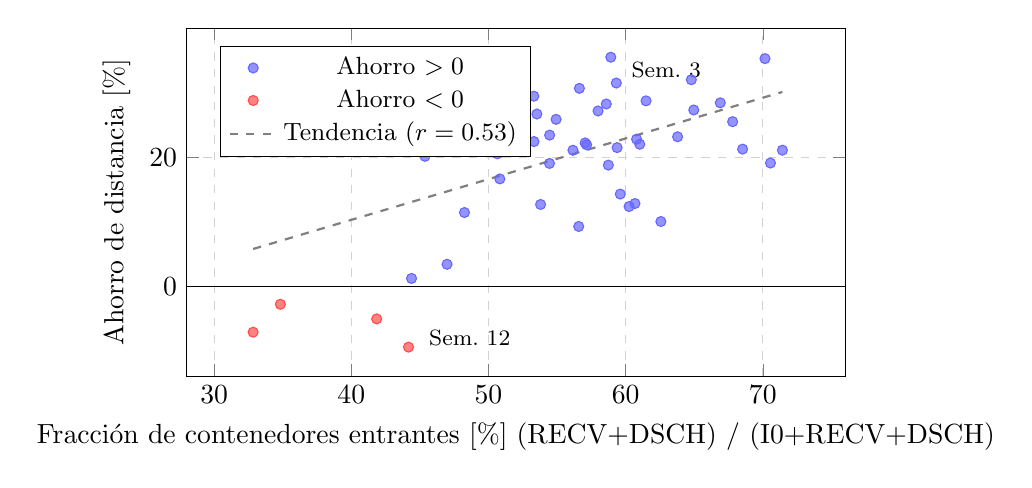
\begin{tikzpicture}
\begin{axis}[
  width=0.82\textwidth, height=6cm,
  xlabel={Fracción de contenedores entrantes [\%] (RECV$+$DSCH) / (I0$+$RECV$+$DSCH)},
  ylabel={Ahorro de distancia [\%]},
  xmin=28, xmax=76,
  ymajorgrids=true, xmajorgrids=true,
  grid style={dashed, gray!35},
  legend style={at={(0.05,0.95)}, anchor=north west, font=\small},
]
% semanas con ahorro positivo
\addplot[only marks, mark=*, mark size=1.8pt, blue!60, fill opacity=0.7]
  coordinates {(54.45,19.02) (48.25,11.41) (58.92,35.48) (46.98,3.39) (54.46,23.41) (66.90,28.41) (50.83,16.62) (71.43,21.07) (60.68,12.81) (50.04,23.05) (60.25,12.34) (62.57,10.02) (58.74,18.76) (64.79,31.99) (53.31,29.44) (59.38,21.47) (56.58,9.25) (64.97,27.30) (63.79,23.15) (56.16,21.06) (58.59,28.23) (61.49,28.72) (45.60,21.40) (53.80,12.66) (54.93,25.85) (57.05,22.20) (39.78,28.68) (60.80,22.78) (56.63,30.66) (44.39,1.20) (48.18,25.79) (59.61,14.27) (51.01,32.12) (57.16,21.90) (68.53,21.24) (53.32,22.41) (70.56,19.08) (44.12,23.13) (70.16,35.26) (50.52,23.90) (61.03,21.99) (50.65,20.51) (45.37,20.12) (57.99,27.15) (67.80,25.49) (52.52,23.85) (59.32,31.48) (53.53,26.68)};
% semanas con ahorro negativo
\addplot[only marks, mark=*, mark size=1.8pt, red!70, fill opacity=0.7]
  coordinates {(44.17,-9.45) (34.83,-2.81) (41.85,-5.07) (32.84,-7.13)};
% línea de tendencia
\addplot[dashed, gray, thick]
  coordinates {(32.84,5.76) (71.43,30.10)};
\addlegendentry{Ahorro $>0$}
\addlegendentry{Ahorro $<0$}
\addlegendentry{Tendencia ($r=0.53$)}
% línea horizontal en 0
\addplot[black, thin] coordinates {(28,0) (76,0)};
% anotaciones semanas extremas
\node[font=\footnotesize, anchor=west] at (axis cs:59.72,33.48) {Sem.~3};
\node[font=\footnotesize, anchor=west] at (axis cs:44.97,-7.95) {Sem.~12};
\end{axis}
\end{tikzpicture}
\caption{Relación entre la fracción de contenedores entrantes y el ahorro de distancia
del modelo respecto a la operación real (52 semanas). Puntos azules: semanas con
reducción positiva; puntos rojos: semanas en que el modelo supera a la operación real en distancia.}
\label{fig:entrantes-vs-ahorro}
\end{figure}